\section{Tidlig konfigurationstabel}
En konfiguration af et system er en kombination af elementer, og en konfigurationstabel beskriver den konfiguration.

Denne beskrivelse er baseret på  \citet[Afsnit 3.2, Side 16-21]{art:essence}.

Systemets `use context' er at systemet bruges til at informere unipolare og bipolare patienter om der har været åbenbare adfærdsændringer. Udfordringen er så om mobilen kan bruges til at gøre dette ved hjælp af sensorer på mobilen.

Den øverste række i \cref{tidlig_konfigurationstabel} navngiver de fire Views i Essence: Paradigm, Product, Project og Process.

`Focus' rækken repræsenterer de største problemer og løsninger i projektet. 
Udfordringen er tiltænkt til at være om man kan bruge en mobil til at overvåge adfærd af psykisk syge og se om den ændrer sig. 
Use context er så tiltænkt at de psykiske syge bruger deres mobil i deres hjem og andre vante omgivelser. 
Så er det tiltænkt at product affordance er at adfærdsdata bruges til at estimere patientens sindstilstand, med den mulighed at denne data kan deles med andre som kan bruge denne data til at hjælpe behandlingen. 
Løsnings strategien er så at bruge en smartphone, og udvikle et system som kan registrere data fra forskellige sensorer for at kompensere for subjektive data der vides om sygdomsforløbet..
Data den indsamler skal være objektiv, så idéen er at den skal fungere som en objektiv dagbog, eller som en fitness tracker der i stedet for at spore fysisk helbred ser på psykisk helbred 

`Overview' rækken repræsenterer projektets stakeholders. 
Hoved perspektivet er selvfølgelig fra patienterne, da det er dem som skal bruge produktet, men der er også sponsorer som er interesseret i at se projektet være en succes såsom Morten, der forslog projektet eller de to i psykologi feltet som der er blevet snakket med. 
Designet på projektet er simpelt idet at der bruges mobil eller wearables til sensor input og at denne data gemmes og analyseres på mobilen, men det kan også tænkes at data skal kunne gemmes på server. 
Argumentet for at lave et sådant projekt er, at depression og mani ofte opdages for sent, hvilket i det fleste tilfælde gør situationen værre.
Hvis symptomerne identificeres så perioden opdages tidligt kan den måske forhindres, hvilket kan spare staten en del udgifter til behandlinger og indlæggelser.
Der er dog det problem at en stor mængde sensorer er nødvendige.
Da systemet er mere tiltænkt at supplere sensor kilder, er dette ikke et så stort problem.
For at evaluere systemets funktionalitet kan der bruges fokusgrupper for at finde ud af om den overholder dogmeregler fra Morten, hvilke kan ses i \cref{app:dogmeregler}.

`Details' rækken repræsenterer nøgle scenarier, nøgle komponenter og features.
Desuden indeholder det sidste felt i denne række også de findings.
Findings er dog speciel i forhold til resten af tabellen, da den skal bruges til at evaluere mulige problemer med den nuværende konfiguration og bruges til som et input til den næste Sprint Planning aktivitet, se \citet[Afsnit 8.5, Side 54]{art:essence}. 
Findings kommer som et resultat af evaluering af systemet. 
Disse findings kunne muligvis være potentielle problemer med plads og batteriforbrug, at der kan være huller i data og at persondataloven kan have noget af sige om den data der indsamles, men dette vides ikke før systemet er blevet evalueret. 

\begin{figure}
	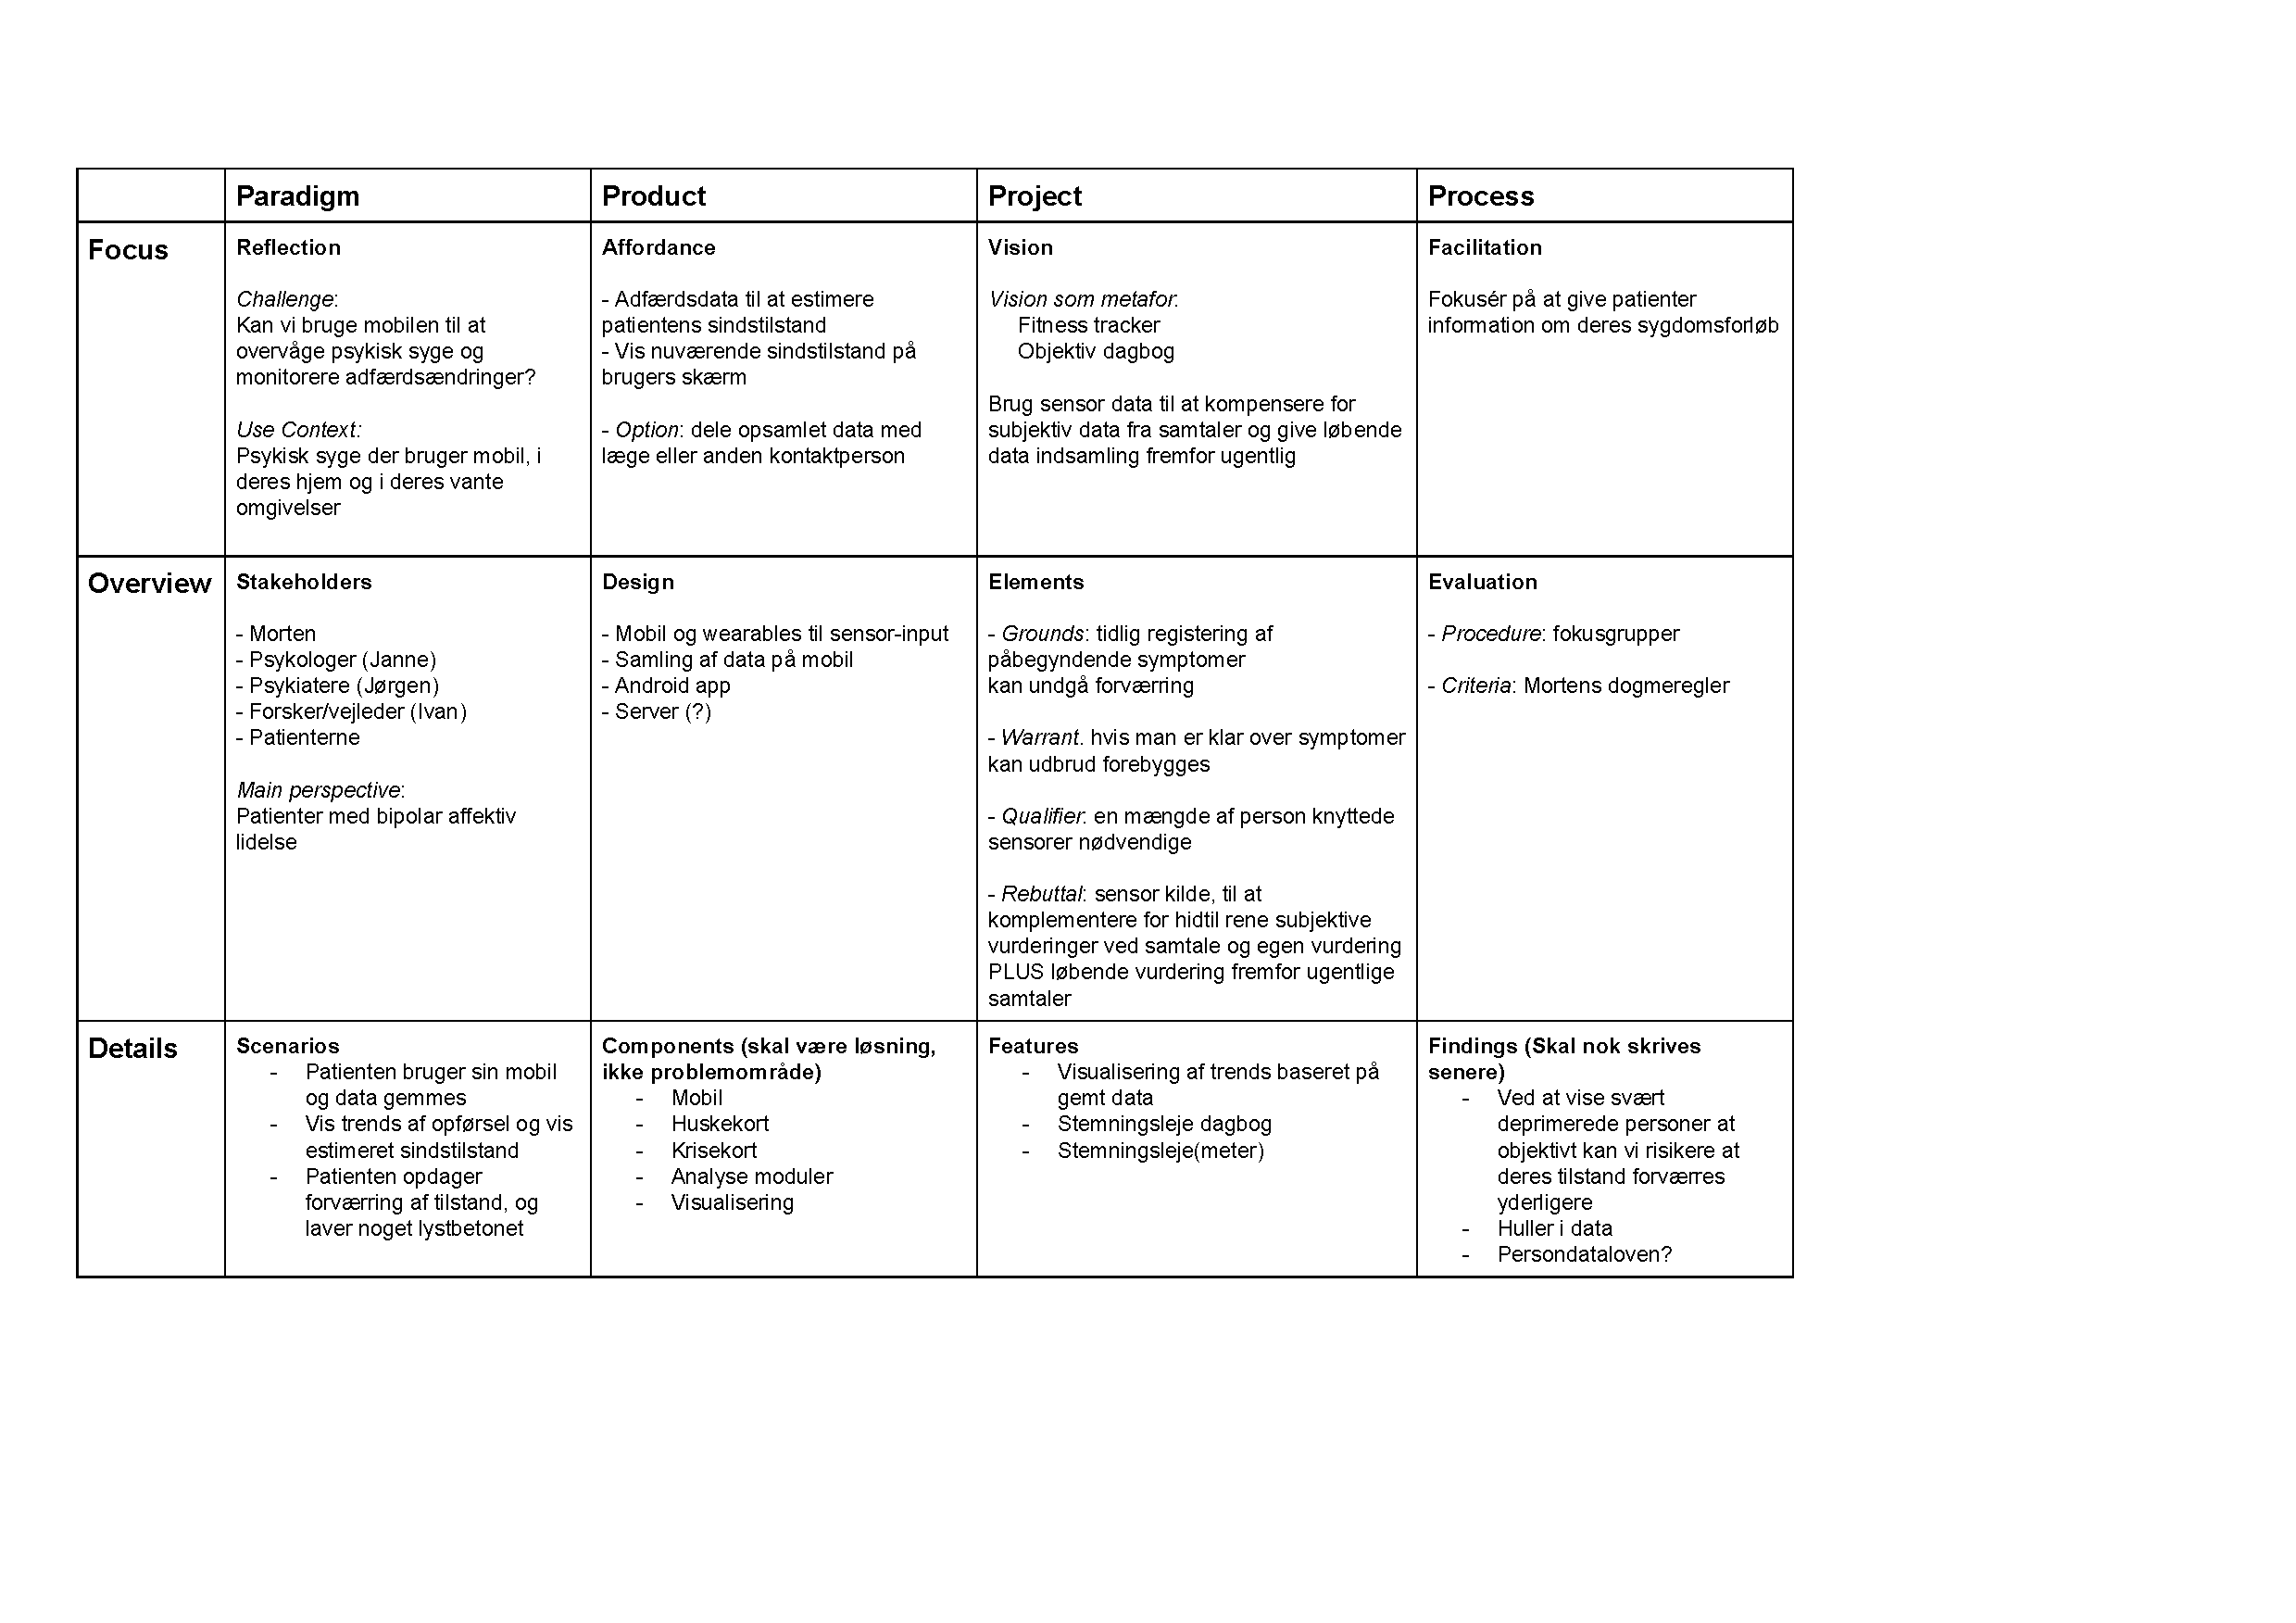
\includegraphics[scale = 0.65,trim = 1cm 3cm 6cm 2cm, angle = 90, clip]{tidlig_konfigurationstabel}
	\caption{Den tidlige konfigurationstabel.}
	\label{tidlig_konfigurationstabel}
\end{figure}